\graphicspath{{chapters/17/images/}}
\chapter{Monte Carlo methods}

\section{Introduction}
Monte Carlo methods are based on games of chance.
The basic idea is to evaluate the value of integrals, for example:

$$I = \int_0^1dx\int_0^{\sqrt{1-x^2}}dy = \frac{\pi}{4}$$

This is done when analytical methods cannot be applied.

	\subsection{Central limit theorem}
	This method is important in statistical mechanics as the aim is to evaluate integrals that define the average value of a quantity.
	Let $f$ be a distribution function such that:

	$$f(x)\ge 0\qquad \int f(x)dx = 1$$

	And $\phi$ an arbitrary function.
	The integral that has to be evaluated to obtain the average value:

	$$I = \int dx\phi(x)f(x)\equiv\langle\phi\rangle_f$$

	Let $x_1, \dots, x_M$ n-dimensional vectors sampled from $f(x)$.
	Then by the central limit theorem:

	$$\tilde{I}_M = \frac{1}{M}\sum\limits_{i=1}^M\phi(x_i)\qquad \lim\limits_{M\rightarrow\infty}\tilde{I}_M = I$$

	Now the average is a good estimator for the integral with some error considering the fluctuation of the function $\phi$ sampled by $f$:

	$$\int dx\phi(x)f(x) = \frac{1}{M}\sum\limits_{i=1}^M\phi(x_i)\pm\frac{1}{\sqrt{M}}\bigl[\langle\phi^2\rangle_f-\langle\phi\rangle_f^2\bigr]^{\frac{1}{2}}$$

	In this way beside a good estimate of the integral also the error can be evaluated.
	So increasing the number of points decreases the error.

	\subsection{Sampling distributions}
	Random number generators are fundamental during Monte Carlo simulations.
	Consider a one dimensional distribution function:

	$$\int_a^bf(x)dx = 1\qquad f(x)\ge 0$$

	The cumulative probability is defined as:

	$$P(X) = \int_a^X f(x)dx\qquad X\in[a,b]$$

	$P(X)$ is the probability that any chosen $x$ from the distribution $f(x)$ lies in $[a, X]$.
	$P(X)$ is a monotonically increasing function of $X$, moreover:

	$$f(X) = \frac{dP}{dX}$$

	Performing a variable transformation $x\rightarrow y$ with $y = g(x)$ a non decreasing function of $x$:

	$$X\ge x \Rightarrow g(X) \ge g(x)$$

	Defining $\tilde{P}(Y=g(X))$ as the probability that $g(X)=Y\ge y\ge g(x)$ is the probability that $X\ge x$, then:

	$$\tilde{P}(Y) = P(X)$$

	This allows to obtain random number distributed according to any distribution starting from any other.
	As an example:

	$$w(r) = \begin{cases}1 &0\le r\le 1\\0 &otherwise\end{cases}\qquad W(\xi) = \int_0^\xi w(r)ds = \begin{cases}0 & \xi<0\\\xi & 0\le\xi\le1\\1 &otherwise\end{cases}$$

	$W(\xi) = \xi$ is the probability that a value of $r$ that has been chosen randomly lies in $[0, \xi]$.
	Now the function $g$ has to be found such that $r = g(x)$ with $g(x)$ a non decreasing function: solve $P(X) = \xi$.

		\subsubsection{An example}
		Assume that random number has to be obtained using the function:

		$$f(x) = ce^{-cx}\qquad x\in[0, +\infty[$$

		Now computing the cumulative distribution function that corresponds to that distribution function and then assuming that $P(X) = \tilde{P}(Y)$, the cumulative distribution function for the uniform random number that was equal to $\xi$.
		In this way the relation between $X$ and $\xi$ is found.

		$$P(X) = \int_0^Xce^{-cx}dx = 1- e^{-cX} = \xi\Rightarrow X = -\frac{1}{C}\ln(1-\xi)$$

		Now any number obtained from the uniform distribution function is the value of $\xi$, which if it is plugged into the previous equation the number distributed according to the desired distribution is obtained.
		The same procedure can be generalized to more than one random variable easily when $f(x)$ is separable into a product of $n$ single-variable distributions.
		This is the procedure that most of the integrator employs to generate velocities and initial conditions to the momenta.

	\subsection{Importance sampling}
	Going back to the problem of the integral.
	Let $I$ be the integral of an observable $\phi$.

	$$I = \int dx\phi(x)f(x) = \int dx\biggl[\frac{\phi(x)f(x)}{h(x)}\biggr]h(x) = \int dx\psi(x)h(x)$$

	Let $h$ be another distribution function defining $\psi(x) = \frac{\phi(x)}{h(x)}$.
	Applying the central limit theorem:

	$$I = \int dx\psi(x)h(x) = \frac{1}{M}\sum\limits_{i=1}^M\psi(x_i)\pm\frac{1}{\sqrt{M}}[\langle\psi^2\rangle_h-\langle\psi\rangle_h^2]^{\frac{1}{2}}$$

	This is done because $h(x)$ might be easier to sample or it might behave better than $f(x)$.
	In the canonical ensemble for example it is better to compute first the Boltzmann-Weight of the conformation before sampling the conformation from the distribution function.
	Another distribution function is used instead of the original, so the optimal choice for this probability distribution function $h(x)$:

	$$\sigma^2[h] = \int dx\psi^2(x)h(x) - \biggl[\int dx\psi(x)h(x)\biggr]^2 = \int dx\frac{\phi^2(x)f^2(x)}{h(x)}-\biggl[\int dx\phi(x)f(x)\biggr]^2$$

	Minimize the functional $\sigma^2[h]$ with the constraint $\int dx h(x) = 1$ driven by the normalization of $h(x)$.
	To do so the methods of	Lagrange multiplier is used introducing an extra variable $\lambda$ and introducing the functional: $F[h] = \sigma^2[h]-\lambda\int dxh(x)$.
	Taking the functional derivative: $\frac{\delta F[h]}{\delta h(x)} = 0$ with $\delta F[h] = F[h+\delta h]-F[h]$ will allow to find an equation for $\lambda$ that will be made explicit using the normalization condition.
	The equality equal to $0$ to minimize $\sigma^2[h]$.
	Now using the Taylor expansion of the first factor on $\delta h$:

	\begin{align*}
		\delta F[h] &= \int dx\biggl[\frac{\phi^2(x)f^2(x)}{h(x) + \delta h(x)} - \frac{\phi^2(x)f^2(x)}{h(x)}\biggr]-\lambda\delta h(x)=\\
								&=-\frac{\phi^2(x)f^2(x)}{h^2(x)}\delta h(x)-\lambda\delta h(x)
	\end{align*}

	Now taking the derivative equal to $0$ an equation to obtain $h$ is found:

	$$\frac{\delta F[h]}{\delta h(x)} = 0\Rightarrow\frac{\phi^2(x)f^2(x)}{h^2(x)}+\lambda = 0\Rightarrow h(x) = \frac{1}{\sqrt{-\lambda}}\phi(x)f(x)$$

	Looking at the normalization condition:

	$$\int dxh(x) = 1\Rightarrow\sqrt{-\lambda} = \int dx\phi(x)f(x) = I$$

	So the optimal choice is $h(x) = \frac{\phi(x)f(x)}{I}\Rightarrow \sigma^2[h] =0$.
	Where $h$ is the function used in importance sampling.
	$I$ is needed, but it is the objective of this computation.
	This means that the true function $h$ cannot be obtained, but there are some tricks to generate a number of points distributed to the function $h$.
	This is called importance sampling and to sample the phase space according to the optimal choice of the distribution function the Metropolis algorithms will be used.
	In this way sampling is efficient and the estimate is a good one.
	A system will be simulated and points distributed according to $h$ will be extracted.

		\subsubsection{An example}
		Computing the integral:

		$$\int_0^1 dxe^{-x}$$

		It can be seen how the function to be integrate is the solid line ($\phi(x)$) in the left panel of figure \ref{fig:importance-sampling-example}.
		Two importance functions can be found: $1-x$ for the dotted line and $1-0.64x$ for the dashed one.
		Looking at the two functions using importance sampling convergence will be faster.
		Looking at the middle panel the result of sampling from $0$ and $1$ uniformly looking at the estimator of the integral.
		There are huge fluctuation.
		Using instead one of the two functions the convergence will be improved as in the right panel the fluctuation are much smaller.

		\begin{figure}[h]
			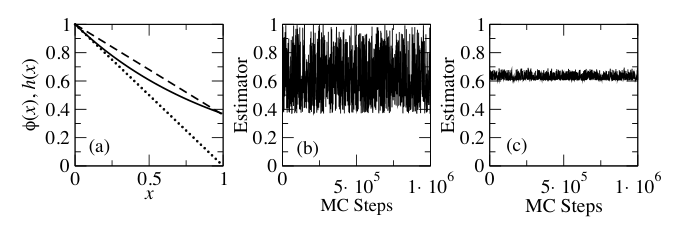
\includegraphics[width=\textwidth]{importance-sampling}
			\caption{The integrand and two possible importance functions}
			\label{fig:importance-sampling-example}
		\end{figure}

	\subsection{Molecular dynamics and Monte Carlo methods}
	In molecular dynamics:

	\begin{multicols}{2}
		\begin{itemize}
			\item All particles move at once, but the $\Delta t$ is usually quite small.
			\item Information on dynamics are available.
			\item Parallel architectures: molecular dynamics is more parallelizable and it is naturally implemented on parallel computers.
		\end{itemize}
	\end{multicols}

	In Monte Carlo:

	\begin{multicols}{2}
		\begin{itemize}
			\item There is no limit on the range of moves: the only limit is the Boltzmann weights, but also unphysical moves can be considered.
				The dynamics of the movement is not important.
			\item Natural thermostats and barostats: they are easily implemented in a Monte Carlo simulation.
			\item Flexibility: it can be applied to any possible system, playing with the moves makes it extremely flexible.
			\item Ergodicity can be achieved thinking about a strange move that moves in the phase space.
		\end{itemize}
	\end{multicols}

\section{Markov chains}
A Markov chain is a rule to obtain the point at the next iteration starting from a point.
The state of the system depends only on the previous instant of time.
The vectors $x_1, x_2, \dots, x_M$ can be generated sequentially in a Markov chain: a rule to generate $x_{i+1}$ given $x_i$ is given.
This points will be sampled according to the same distribution from which we want to sample:

$$\tilde{I}_M = \frac{1}{M}\sum\limits_{i=1}^M\phi(x_i)$$

This rule is defined as $R(x|y)$,  the probability to obtain $x$ given $y$.
If there are two micro states it is the probability to move to a microstate $x$ from a microstate $y$.

	\subsection{Detailed balance condition}
	To define a rule a detailed balance condition is imposed

	$$R(x|y)f(y) = R(y|x)f(x)$$

	This means that the probability to go from $y$ to $x$ times the probability of being in $y$  is equal to the inverse movement.
	Some features of the detailed balance condition are:

	\begin{itemize}
		\item It represents microscopic reversibility.
		\item It is an unbiased sampling of phase space.
		\item It is sufficient but not strictly necessary condition to ensure proper sampling of phase space.
			Unbiased sampling can be obtained without the detailed balance condition.
	\end{itemize}

	\subsection{Rejection methods}
	Using the detailed balance condition a rejection method is built.
	Let $T(x|y)$ a rule to generate a trial move or proposed move from $y$ to $x$.
	This is the probability to go from $y$ to $x$ by the way the proposed move are constructed.
	This quantity is normalized:

	$$\int dxT(x|y) = 1$$

	So the probability to go from state $y$ to anywhere is $1$.
	Let $A(x|y)$ be the probability to accept the move from $y$ to $x$.
	Now the probability to go from $y$ to $x$ is the product of the probability of generating the move and the probability of accepting that move:

	$$R(x|y) = A(x|y)T(x|y)$$

	By applying the detailed balance condition:

	$$A(x|y)T(x|y)f(y) = A(y|x)T(y|x)f(x)$$

	By looking at this equation it can be seen how the acceptance probabilities are related.
	In this way the integral is cancelled because it is at the denominator for $f$.
	If the algorithm is symmetrical the probability of the inverses moves is equal.
	The acceptance probability are related to each other and are not independent.
	Writing down this relation:

	$$A(x|y) = \frac{T(y|x)f(x)}{T(x|y)f(y)}A(y|x) = r(x|y)A(y|x)$$

	Where $\frac{T(y|x)f(x)}{T(x|y)f(x)} = r(x|y)$.
	If $A(x|y) = 1$ the move $y\rightarrow x$ is favoured $\Rightarrow A(y|x)< 1 \Rightarrow r(x|y)>1$.
	If $A(x|y) < 1$, $y\rightarrow x$ is not entirely favoured $\Rightarrow A(y|x) = 1\Rightarrow r(x|y) < 1$.
	Writing down this $A$ can be defined as:

	$$A(x|y) = \min[1, r(x|y)]$$

	So the acceptance probability of the move from $y$ to $x$ is the minimum between $1$ and $r(x|y)$.

	\subsection{Metropolis algorithm}
	In order to build the acceptance rate the trial distribution $T(x_{k+1}|x_k)$ has to be written to be able to propose a move $x_k\rightarrow x_{k+1}$ and there is a need to be able to compute:

	$$r(x_{k+1}|x_k) = \frac{T(x_k|x_{k+1})f(x_{k+1})}{T(x_{k+1}|x_k)f(x_k)}$$

	If $r(x_{k+1}|x_k)>1$ accept the move, otherwise accept the move with probability given by $r(x_{k+1}|x_k)$: extract a random number $\xi\in[0,1]$.
	If $\xi< r(x_{k+1}|x_k)$ accept the move.
	Rejections do count: when a move is rejected that particular conformation will be counted twice because the importance sampling samples the system with a distribution function that is required by it, which means that points that are more representative for the representation functions will be explored more: if a move if rejected that point counts more in the average.

		\subsubsection{Proof}
		Let the associated probability for each point $x_1, \dots, x_n$: $\pi_1(x), \dots, \pi_n(x)$.
		With a huge number of moves the probability is equal to the desired distribution.

		$$\lim\limits_{n\rightarrow\infty}\pi_n(x) = f(x)$$

		Proof by recursive relation: $\pi_{n+1}(x)$ receives contributions from accepted moves starting at $y$ and ending in $x$ and from attempted moves to $y$ that are rejected:

		$$\pi_{n+1}(x) = \int A(x|y)T(x|y)\pi_n(y)dy + \pi_n(x)\int[1-A(y|x)]T(y|x)dy$$

		If $\pi_n(x) = f(x)$:

		$$\pi_{n+1} = \int A(x|y)T(x|y)f(y)dy + f(x)\int[1-A(y|x)]T(y|x)dy$$

		Considering the detailed balance condition: $A(x|y)T(x|y)f(y) = A(y|x)T(y|x)f(x)$ two terms cancel each other out:

		$$\pi_{n+1}(x) = f(x)\int T(y|x)dy = f(x)$$

		So if the system arrives at the distribution function $f$ it will stay there.

		\subsubsection{Summary}
		Everything sums up to evaluate the ratio of the final over probabilities of generating the moves to the initial and final states.

		$$r(x|y) = \frac{T(y|x)f(x)}{T(x|y)f(y)}$$

		The acceptance probability is computed according to:

		$$A(x|y) = \min[1, r(x|y)]$$

		For a uniform choice of $T(x|y)$, so the same probability from $x$ to $y$ and from $y$ to $x$:

		$$r(x|y) = \frac{f(x)}{f(y)}\Rightarrow A(x|y) = \min\biggl[1, \frac{f(x)}{f(y)}\biggr]$$

		Considering the Boltzmann distribution in this ratio the partition function would be cancelled.

	\subsection{Canonical distribution}
	In the canonical distribution the partition function, where the integrand is the Boltzmann weight:

	$$Q(N, V, T) = \frac{1}{N!\lambda^{3N}}\int d\vec{r}_1\cdots d\vec{r}_Ne^{-\beta U(\vec{r}_1, \dots, \vec{r}_N)}$$

	So the acceptance probability for a move from $r$ to $r'$ will be:

	$$A(r'|r) = \min\bigl[1, e^{-\beta(U(r')-U(r))}\bigr]$$

	$\Delta U < 0$ accept the move, so when decreasing the energy the move is accepted.
	$\Delta U > 0$ accept the move with probability $e^{-\beta\Delta U}$ if the energy has increased.
	In this way points that are distributed according to Boltzmann distribution can be simulated.
	Considering the acceptance, the Monte Carlo method will be efficient for an acceptance rate neither too high (not exploring enough) nor to low (never moving).
	The acceptance probability depends on the energy difference.
	Changing the coordinates of all the particles randomly it is highly probable to generate a huge energy difference (energy is an extensive quantity), causing the acceptance rate to be small.
	Because of this it is better to move the particles one by one.
	The particle to be updated should be chosen randomly because, when doing it sequentially the reverse move has not the same probability so the probability will not be symmetrical.
	A Monte Carlo pass is equivalent to $N$ trial moves: particles must be chosen randomly.
	On average each particle has seen at least one attempt to be moved.
	Considering a possible trial move:

	$$\begin{cases}x'_i = x_i+\frac{1}{\sqrt{3}}(\xi_x-0.5)\Delta\\y'_i = y_i+\frac{1}{\sqrt{3}}(\xi_y-0.5)\Delta\\z'_i = z_i+\frac{1}{\sqrt{3}}(\xi_z-0.5)\Delta\end{cases}$$

	Where $\xi$ is the random number, and the $0.5$ is needed to generate forward and backward moves, centring it around zero so to have the same probability to generate the backward move (when it is less than $0$).
	In one Monte Carlo pass each particle on average has seen one attempt.
	It is not necessary to recompute all the energy $U(r')$ in full at each move, because changing only the coordinates of one particle and taking its list of neighbours, the energy for that particle and list of neighbours are updated.
	$\Delta$ is the magnitude of the movement.
	If it is too big the probability to accept the move will be small.
	If it is too small the phase space is not being explored too well.
	As a rule of thumb after trying of simulation and keeping track of the acceptance rate, a good value should have an acceptance rate between $30$ and $50\%$.

\section{Simulating ensembles}

	\subsection{Isothermal-isobaric ensemble}
	Considering the partition function for the ensemble:

	$$\Delta(N, P, T) = \frac{1}{V_0} \int dVe^{-\beta PV}Q(N, V, T) = \frac{1}{V_0}\frac{1}{N!\lambda^{3N}}\int_0^{\infty}dVe^{-\beta PV}\int_Vd\vec{r}_1\cdots d\vec{r}_Ne^{-\beta U(\vec{r}_1, \dots, \vec{r}_N)}$$

	The scheme is the same as in the canonical ensemble with another trial move on the volume volume: $V' = V + (\xi_V-0.5)\delta$.
	The percentage of volume moves has to be chosen.
	Volume changes imply scaling of particle coordinates: $r'_i = \left(\frac{V'}{V}\right)^{\frac{1}{3}}r_i$.
	Making the dependance on volume explicit:

	$$\Delta(N, P, T) = \frac{1}{V_0}\frac{1}{N!\lambda^{3N}}\int_0^{\infty}dVV^Ne^{-\beta PV}\int_Vd\vec{s}_1\cdots d\vec{s}_Ne^{-\beta U\left(V^{\frac{1}{3}}\vec{s}_1,\dots, V^{\frac{1}{3}}\vec{s}_N\right)}$$

	Now the distribution function is obtained and the acceptance probability will be:

	$$A(V'|V) = \min\bigl[1, e^{-\beta P(V'-V)e^{N\ln \frac{V'}{V}}e^{-\beta(U(r')-U(r))}}\bigr]$$

	$\delta$, the variation on the volume, should be small to accept the move because if inflating the system too much the difference in energy would be huge.
	This is computational demanding because the coordinates of all the particles are being changed so the force has to be recomputed for all of them, so it is less frequent with higher acceptance.

	\subsection{Gran canonical ensemble}
	In Monte Carlo simulations in the grand canonical ensemble can be performed.
	Considering the partition function:

	$$\mathcal{E}(\mu, V, T) = \sum\limits_{N=0}^{\infty}e^{\beta\mu N}Q(N, V, T) = \sum\limits_{N+0}^{\infty}e^{\beta\mu N}\frac{1}{N!\lambda^{3N}}\int d\vec{r}_1\cdots d\vec{r}_Ne^{-\beta U(\vec{r}_1, \dots, \vec{r}_N)}$$

	So a move of the coordinates is the previous scheme with with trial moves with particle insertion and particle deletion.
	Considering particle insertion:

	$$A(N+1|N) = \min\biggl[1, \frac{V}{\lambda^3(N+1)}e^{\beta\mu}e^{-\beta(U(r')-U(r))}\biggr]$$

	Considering particle deletion:

	$$A(N-1|N) = \min\biggl[1, \frac{\lambda^3V}{V}e^{-\beta\mu}e^{-\beta(U(r')-U(r))}\biggr]$$

	Now it can be simulated at constant chemical potential.
	This is not so expensive: $U(r')$ requires only the change in energy due to one particle.

\section{Hybrid Monte Carlo}
Hybrid Monte Carlo is a technique in which both Monte Carlo and molecular dynamics are used.
Molecular dynamics is used as an engine to generate Monte Carlo moves:
This is useful so that it can be tried to use a very big $\Delta t$ in molecular dynamics, generating new coordinates and momenta and using the metropolis criterion the moves will be accepted or not.
In this way the correctness of the move is determined by the acceptance probability.

$$A(r', p' | r, p) = \min\{1, e^{-\beta[\mathcal{H}(r', p')-\mathcal{H}(r, p)]}\} = \min\bigl[1,e^{-\beta\Delta\mathcal{H}}\bigr]$$

If the algorithm in molecular dynamics is symplectic and time-reversible algorithm:

$$T(r', p'|r, p) = T(r, -p|r', -p')$$

One move is quite expensive, so it is better to have a higher acceptance rate between $40$ and $70\%$.
In the case of a rejected move $p$ is re-sampled to obtained a new move as Molecular Dynamics is deterministic.
If the integrator is time-reversible the detailed balance holds.

	\subsection{Detailed balance}
	The detailed balance condition or the result is:

	$$\int d^Npd^Np' T(r',p'|r,p)A(r',p'|r,p)f(r,p) = \int d^Npd^Np'T(r, p|r',p;)A(r,p|r',p')f(r',p')$$

	Considering the acceptance rate and the distribution:

	$$A(r',p'|r,p)f(r,p) = \frac{1}{Q_N(V, T)}\min\bigl[1, e^{-\beta(\mathcal{H}(r', p')-\mathcal{H}(r,p))}\bigr]e^{-\beta\mathcal{H}(r, p)}$$

	Multiplying inside the Boltzmann weight:

	$$A(r',p'|r,p)f(r,p) = \frac{1}{Q_N(V, T)}\min\bigl[e^{-\beta\mathcal{H}(r, p)}, e^{-\beta\mathcal{H}(r', p')}\bigr]$$

	Similarly:

	$$A(r,p|r',p')f(r,'p') = \frac{1}{Q_N(V, T)}\min\bigl[e^{-\beta\mathcal{H}(r', p')}, e^{-\beta\mathcal{H}(r, p)}\bigr]$$

	Therefore:

	$$A(r', p'|r, p)f(r, p) = A(r, p|r', p')f(r',p')$$

	So that:

	$$A(r',p'|r,p)f(r,p) = \frac{1}{Q_N(V, T)}\min\bigl[1, e^{-\beta(\mathcal{H}(r', p')-\mathcal{H}(r,p))}\bigr]e^{-\beta\mathcal{H}(r, p)}$$

	Using the property of the symplectic time-reversible algorithm, inverting the velocities the movement is reversed.

	$$T(r', p'|r, p) = T(r, -p|r', -p')$$

	Substituting this into the second integral:

	$$\int d^Npd^Np'T(r',p'|r, p)A(r', p'|r, p)f(r,p) = \int d^Npd^Np'T(r, -p|r', -p')A(r, p|r', p')f(r', p')$$

	Performing a change of variables: $p, p'\rightarrow -p, -p'$:

	$$\int d^Npd^Np'T(r',p'|r, p)A(r', p'|r, p)f(r,p) = \int d^Npd^Np'T(r,p|r', p')A(r, p|r', p')f(r',p')$$

	In this way the detailed balance condition is satisfied.
